% LTeX: de-DE
\nomenclature[G]{\(\alpha_e\)}{Auslenkungswinkel der Erregerschwingung\nomunit{\rad}}%
\nomenclature[L]{\(\hat{M}_e\)}{Externes Drehmoment\nomunit{\newton\metre}}
\nomenclature[G]{\(\varphi_1\)}{Auslenkungswinkel Rotor 1\nomunit{\rad}}
\nomenclature[G]{\(\varphi_2\)}{Auslenkungswinkel Rotor 2\nomunit{\rad}}
\nomenclature[L]{\(b^\ast\)}{Dämpfung (Wirbelstrombremse)\nomunit{\newton\metre\second}}
\nomenclature[L]{\(D^\ast\)}{Torsionsfederkonstante 1\nomunit{\newton\metre}}
\nomenclature[L]{\(D^{\ast\ast}\)}{Torsionsfederkonstante 2\nomunit{\newton\metre}}
\nomenclature[L]{\(DD^\ast\)}{Kopplungsfederkonstante\nomunit{\newton\metre}}
\nomenclature[L]{\(J\)}{Trägheitsmoment\nomunit{\kilo\gram\metre\squared}}
\nomenclature[G]{\(\omega_e\)}{Erregerfrequenz\nomunit{\rad\per\second}}
\nomenclature[G]{\(\omega_0\)}{Eigenfrequenz\nomunit{\rad\per\second}}
\nomenclature[G]{\(\omega_R\)}{Resonanzfrequenz\nomunit{\rad\per\second}}
\nomenclature[G]{\(\xi\)}{Phasenverschiebung\nomunit{1}}
\nomenclature[G]{\(\delta\)}{Dämpfungskoeffizient\nomunit{\newton\metre\second}}
\nomenclature[L]{\(r_z\)}{Abstand Zusatzmasse von Achse\nomunit{\metre}}
\nomenclature[L]{\(m_z\)}{Masse der Unwucht\nomunit{\kilo\gram}}
\nomenclature[L]{\(r_1\)}{Bahnkurve Rotor 1\nomunit{\metre}}
\nomenclature[L]{\(r_2\)}{Bahnkurve Rotor 2\nomunit{\metre}}
\chapter{Simulationsaufgabe}
    Das in \textsc{MATLAB} zu erstellende Simulationsprogramm soll die Bewegung des Systems (frei und
    erzwungen) für beliebige Anfangsbedingungen berechnen und typische Eigenschaften in übersichtlicher Form grafisch
    darstellen können.

    \section{Aufgabenstellung III}

        Es soll der Einfluss einer Zusatzmasse auf die erzwungenen Schwingungen des Systems numerisch untersucht werden.
        Insbesondere sollen kritische Parameterintervalle ermittelt werden, die zu instabilen, mitunter auch chaotischen Schwingungen führen.
        Der Einfluss der Zusatzmasse auf das Trägheitsmoment wird hierbei vernachlässigt.
        Das zu modellierende physikalische System besteht aus zwei über eine Spiralfeder miteinander gekoppelte, auf einer gemeinsamen Achse sitzenden Torsionspendel (siehe \cref{Prinzipskizzen}). Beide Pendel sind in allen ihren Parametern (Trägheitsmoment, Federkonstante der Rückstellfeder, Reibungskoeffizient) identisch.
        Das System soll sowohl freie wie auch erzwungene Schwingungen variabler Frequenz ausführen können, wobei die äußere Erregung nur an einem Rad angreift.
        Das System lässt sich z.B. durch zwei gekoppelte, auf einer Achse laufenden Pohl'schen Rädern (siehe \cref{Aufbau Pohl'sches Rad}) realisieren, wobei nur eines mit einem externen Erregermoment versehen ist.
        Die Modellierung der Bewegung des Systems soll mit folgendem Parameterset auskommen: Trägheitsmoment \(J\), Torsionsfederkonstante der beiden Rückstellfedern \(D^\ast\) und der Kopplungsfeder \(DD^\ast\), Dämpfungskoeffizient \(b^\ast\).
        Die Auslenkung der beiden schwingenden Systeme wird durch die Winkel \(\varphi_1\) und \(\varphi_2\) beschrieben.
        Die für eine erzwungene Schwingung erforderliche Anregungsschwingung \(\alpha_e(t)\) sei gegeben durch die Funktion:

        \begin{align}
            \alpha_e(t) = \hat{\alpha}_e \sin(\omega_e t)\nonumber
        \end{align}

        Zudem müssen Anfangsbedingungen (AB)

        \begin{align}
            \varphi_1(0) \qquad \dot{\varphi}_1(0)\nonumber
        \end{align}

        sowie

        \begin{align}
            \varphi_1(0) \qquad \dot{\varphi}_1(0)\nonumber
        \end{align}

        vorgegeben werden.\par\medskip

        Für Modellrechnungen werden folgende Parameterwerte verwendet:
        \begin{table}[h]
            \centering
            \caption{Parameter zur Modellberechnung.}\label{tab:params modellberechnung}
            \begin{tabular}{@{}lSl@{}}
                \toprule
                Größe& {Wert}& Einheit\\
                \midrule
                \(J\)& 10& \unit{\kilo\gram\metre\squared}\\
                \(D^\ast\)& 0.1& \unit{\newton\metre}\\
                \(DD^\ast\)& 0.01& \unit{\newton\metre}\\
                \(b^\ast\)& 0.2& \unit{\newton\metre\second}\\
                \(\hat{\alpha}_e\)& 50& \unit{1}\\
                \bottomrule
            \end{tabular}
        \end{table}

        \begin{figure}[htbp]
            \centering
            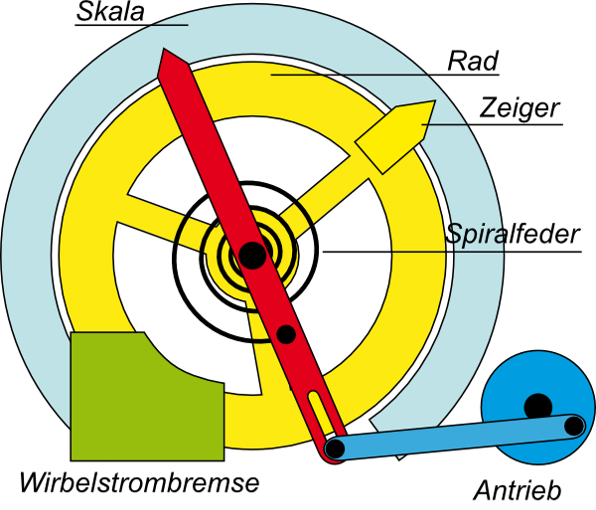
\includegraphics[width=0.6\textwidth]{Bilder/Kapitel-1/Aufbau Pohl'sches Rad.png}
            \caption[Aufbau eines realen pohl'schen Rades]{Aufbau eines realen pohl'schen Rades.}\label{Aufbau Pohl'sches Rad}
            \end{figure}

        \begin{figure}[htbp]
            \begin{subfigure}[c]{0.5\textwidth}
                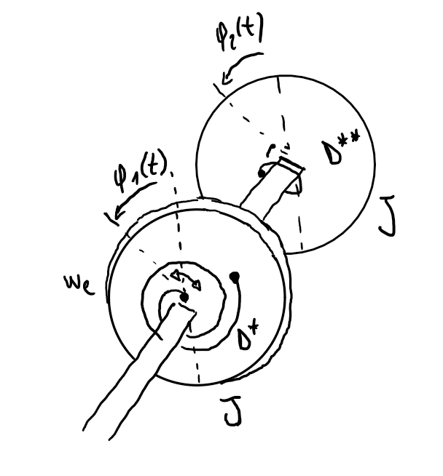
\includegraphics[height=.3\textheight]{Bilder/Kapitel-1/Skizze zwei gekoppelter Torsionspendel.png}
                \subcaption{Skizze zweier gekoppelter Torsionspendel.}
            \end{subfigure}
            \begin{subfigure}[c]{0.5\textwidth}
                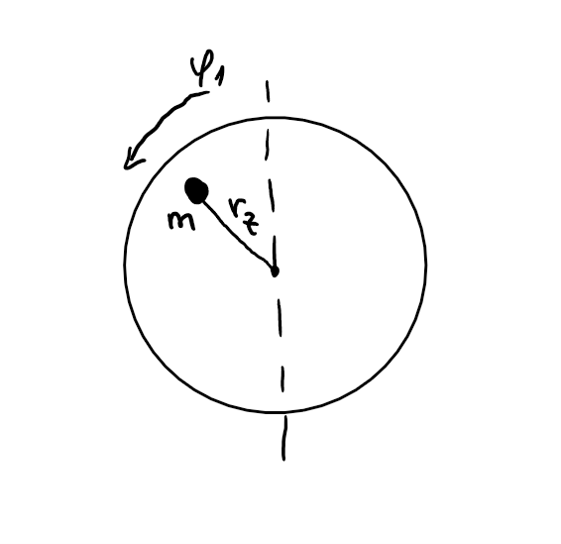
\includegraphics[height=.3\textheight]{Bilder/Kapitel-1/Skizze Torsionspendel 1 mit Zusatzmasse m.png}
                \subcaption{Skizze Torsionspendel 1 mit Zusatzmasse \(m\).}
            \end{subfigure}
            \caption[Prinzipskizzen zweier gekoppelter Torsionspendel]{Prinzipskizzen zweier gekoppelter Torsionspendel. (a) Geometrische Anordnungg mit relevanten Systemgrößen, (b) Skizze der Scheibe mit Zusatzmasse.}\label{Prinzipskizzen}
        \end{figure}

    \section{Leistungsumfang des Programms}

        Das erstellte Programm soll folgende Anforderungen erfüllen:
        \begin{itemize}
            \item Untersuchung des Einflusses einer Unwucht in Form einer Zusatzmasse \(m_Z = \qty{1}{\kilo\gram}\) im Abstand \(r_Z = \qty{0.1}{\metre}\) von der Rotorachse angebracht an der extern erregten Scheibe auf die erzwungenen Schwingungen des Systems anhand einer grafischen Darstellung.
            Insbesondere sollen kritische Parameterintervalle ermittelt werden, die zu instabilen, mitunter auch chaotischen Schwingungen führen.
            \item Animation: Berechnung und grafische Darstellung der Bahnkurven \(r_1(t)\) und \(r_2(t)\) der Rotorzeiger in der x-y-Ebene für frei wählbare Werte der Anfangsbedingungen.
            Die Lage des Startpunktes soll im Diagramm ersichtlich sein.
            \item Angabe aller relevanten festen und variierten Parameter in einem separaten Fenster zusammen mit einem Kurztext, der das momentan laufende, numerische Experiment klassifiziert:
            \begin{itemize}
                \item freie Schwingung,
                \item gedämpfte Schwingung,
                \item erzwungene Schwingung ohne/mit Dämpfung,
                \item mit/ohne Unwucht,
                \item gekoppelte/entkoppelte Schwinger,
                \item analytische/numerische Berechnung.
            \end{itemize}
        \end{itemize}